% !TEX TS-program = pdflatexmk
\documentclass[12pt]{article}

% Layout.
\usepackage[top=1in, bottom=0.75in, left=1in, right=1in, headheight=1in, headsep=6pt]{geometry}

% Fonts.
\usepackage{mathptmx}
\usepackage[scaled=0.86]{helvet}
\renewcommand{\emph}[1]{\textsf{\textbf{#1}}}
\newcommand{\ans}[1][1in]{\rule{#1}{.5pt}}

\usepackage[parfill]{parskip}
\usepackage{adjustbox}

% Misc packages.
\usepackage{amsmath,amssymb,latexsym}
\usepackage{graphicx,hyperref}
\usepackage{array}
\usepackage{xcolor}
\usepackage{multicol,tikz}
\usepackage{tabularx,colortbl,booktabs,xparse}
\usepackage{enumitem}

%\renewcommand{\familydefault}{\sfdefault}

\usetikzlibrary{calc,trees,positioning,arrows,fit,shapes,through, backgrounds}
\usetikzlibrary{patterns}

\newcommand{\be}{\begin{enumerate}}
\newcommand{\ee}{\end{enumerate}}


\NewDocumentCommand{\rot}{O{45} O{1em} m}{\makebox[#2][l]{\rotatebox{#1}{#3}}}%

\usepackage{fancyhdr}
\pagestyle{fancy} 
\lhead{\large\sf\textbf{MATH F113X: Introduction to Scheduling}}
%\chead{}
\rhead{\emph{lecture notes}}

\begin{document}
\emph{Goal} Learn about the following terminology: schedule, digraph, processors, finishing time, optimal finishing time, optimal schedule, idle time, critical path, critical time.\\

\begin{enumerate}
\item \emph{Motivating Example} Fixing a Flat Bike Tire\\

\begin{tabular}{llll}
label&task&time&dependence\\
\hline
A&buy a replacement tube&20 minutes&\\
&patch kit&&\\
B&find tools&5 minutes&\\
C&remove tire and tube&10 minutes&\\
D&replace tire and new tube&10 minutes&\\
E&repair old tube&10 minutes&\\
\end{tabular}
\vfill

\be
\item Schedule with one processor

total time: \ans

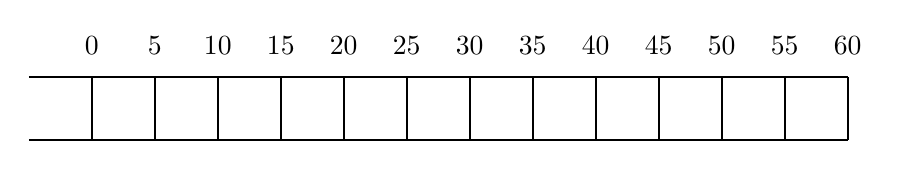
\begin{tikzpicture}[scale =.8]
\foreach \x [evaluate=\x as \xeval using int(\x*5)] in {0,1,...,12}{
	\node  at (\x,1.5){$\xeval$};
	\draw[thick] (\x,0) -- (\x,1);
	}
\foreach \y in {0,1}{\draw[thick] (-1,\y)--(12,\y);}
\end{tikzpicture}


\item Schedule with two processors

total time: \ans


\hspace*{-1in}	\begin{tabular}{c || c}
time &   \quad \hspace{6in} \quad \\ \hline
done& \\ \hline
ready& \\ \hline
\end{tabular}


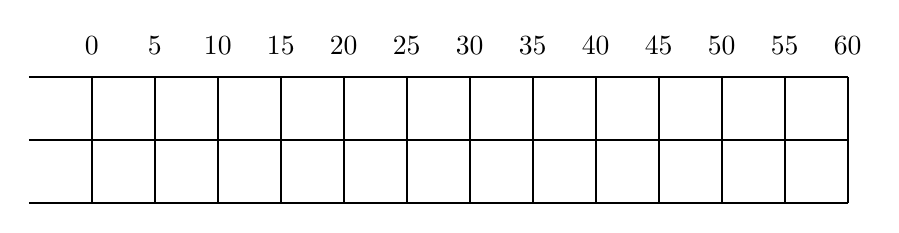
\begin{tikzpicture}[scale =.8]
\foreach \x [evaluate=\x as \xeval using int(\x*5)] in {0,1,...,12}{
	\node  at (\x,2.5){$\xeval$};
	\draw[thick] (\x,0) -- (\x,2);
	}
\foreach \y in {0,1,2}{\draw[thick] (-1,\y)--(12,\y);}
\end{tikzpicture}
\vspace{.3in}

\item Schedule with three processors

total time: \ans


\hspace*{-1in}	\begin{tabular}{c || c}
time &   \quad \hspace{6in} \quad \\ \hline
done& \\ \hline
ready& \\ \hline
\end{tabular}

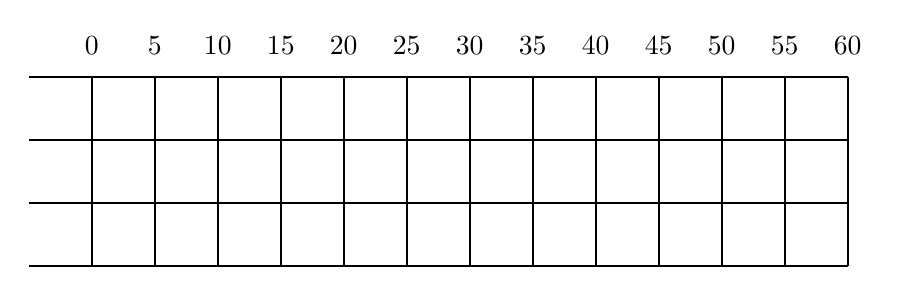
\begin{tikzpicture}[scale =.8]
\foreach \x [evaluate=\x as \xeval using int(\x*5)] in {0,1,...,12}{
	\node  at (\x,3.5){$\xeval$};
	\draw[thick] (\x,0) -- (\x,3);
	}
\foreach \y in {0,1,2,3}{\draw[thick] (-1,\y)--(12,\y);}
\end{tikzpicture}
\ee
\newpage
\item Terminology
	\begin{enumerate}
	\item \emph{schedule}
	\vfill
	\item \emph{digraph}
	\vfill
	\item \emph{processors}
	\vfill
	\item \emph{finishing time}
	\vfill
	\item \emph{optimal finishing time and optimal schedule}
	\vfill
	\item \emph{idle time}
	\vfill
	\item \emph{critical path}
	\vfill
	\item \emph{critical time}
	\vfill
	\end{enumerate}

\item \emph{General Example}: Create a digraph. Make a valid schedule with TWO processors. Determine values of finishing time, idle time and critical time.\\

\begin{tabular}{llll}
label/task&time&dependence\\
\hline
A&2&\\
B&1&\\
C&2&\\
D&3&A\\
E&6&A, B\\
F&8&B, C\\
G&5&E, F\\
\end{tabular}

\hspace*{-1in}	\begin{tabular}{c || c}
time &   \quad \hspace{6in} \quad \\ \hline
done& \\ \hline
ready& \\ \hline
\end{tabular}

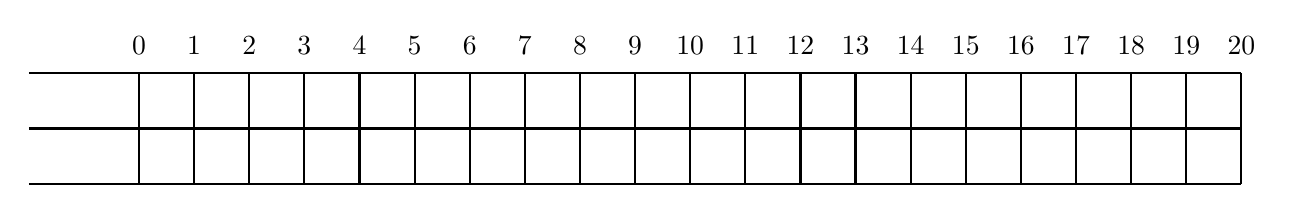
\begin{tikzpicture}[scale=.7]
\foreach \x in {0,1,...,20}{
	\node  at (\x,2.5){$\x$};
	\draw[thick] (\x,0) -- (\x,2);
	}
\foreach \y in {0,1,2}{\draw[thick] (-2,\y)--(20,\y);}
\end{tikzpicture}
\end{enumerate}
\end{document}